\documentclass[12pt]{article}
\usepackage{preamble}

\newcommand{\documenttitle}{Programa de Mantenimiento Aprobado}
\newcommand{\documentsubtitle}{Aeronaves ligeras -- Parte-ML (no comerciales)}
\newcommand{\aircraft}{Socata TB 10 S/N 649}
\newcommand{\groupauthors}{Grupo 7 -- González Pérez, Christian; Alba Buitrón, Guillermo y Gil Getino, Alejandro}
\newcommand{\FH}{FH}
\newcommand{\LDG}{LDG}

\begin{document}

\lfoot{Autor: Grupo 7}
\rfoot{Programa de Mantenimiento Aprobado}

%%%%%%%%%%%%%%%%%%%%%%%%%%%%%%%%%%%%%%%%%%%%%%%%%%%%%
%%%%%%%%%%%%%%%%%%%%% Portada %%%%%%%%%%%%%%%%%%%%%%%
%%%%%%%%%%%%%%%%%%%%%%%%%%%%%%%%%%%%%%%%%%%%%%%%%%%%%

\begin{titlepage}
    \thispagestyle{empty}

    \noindent
    
\includegraphics[width=0.32\textwidth]{Figuras/ule.jpg}
    \hfill
    
\includegraphics[height=2.4cm]{Figuras/escudo-ingenierias.png}

    \vspace{1.2cm}

    \begin{center}
        {\fontsize{17pt}{21pt}\selectfont\bfseries
        Escuela de Ingenierías \\ Industrial, Informática y Aeroespacial
        }

        \vspace{0.9cm}

        {\large\bfseries Mantenimiento y Certificación de Vehículos Aeroespaciales}\\[0.35cm]
        {\large Programa Basado en el Reglamento (UE) N\textordmasculine{} 1321/2014 -- Parte-ML}

        \vspace{1.0cm}

        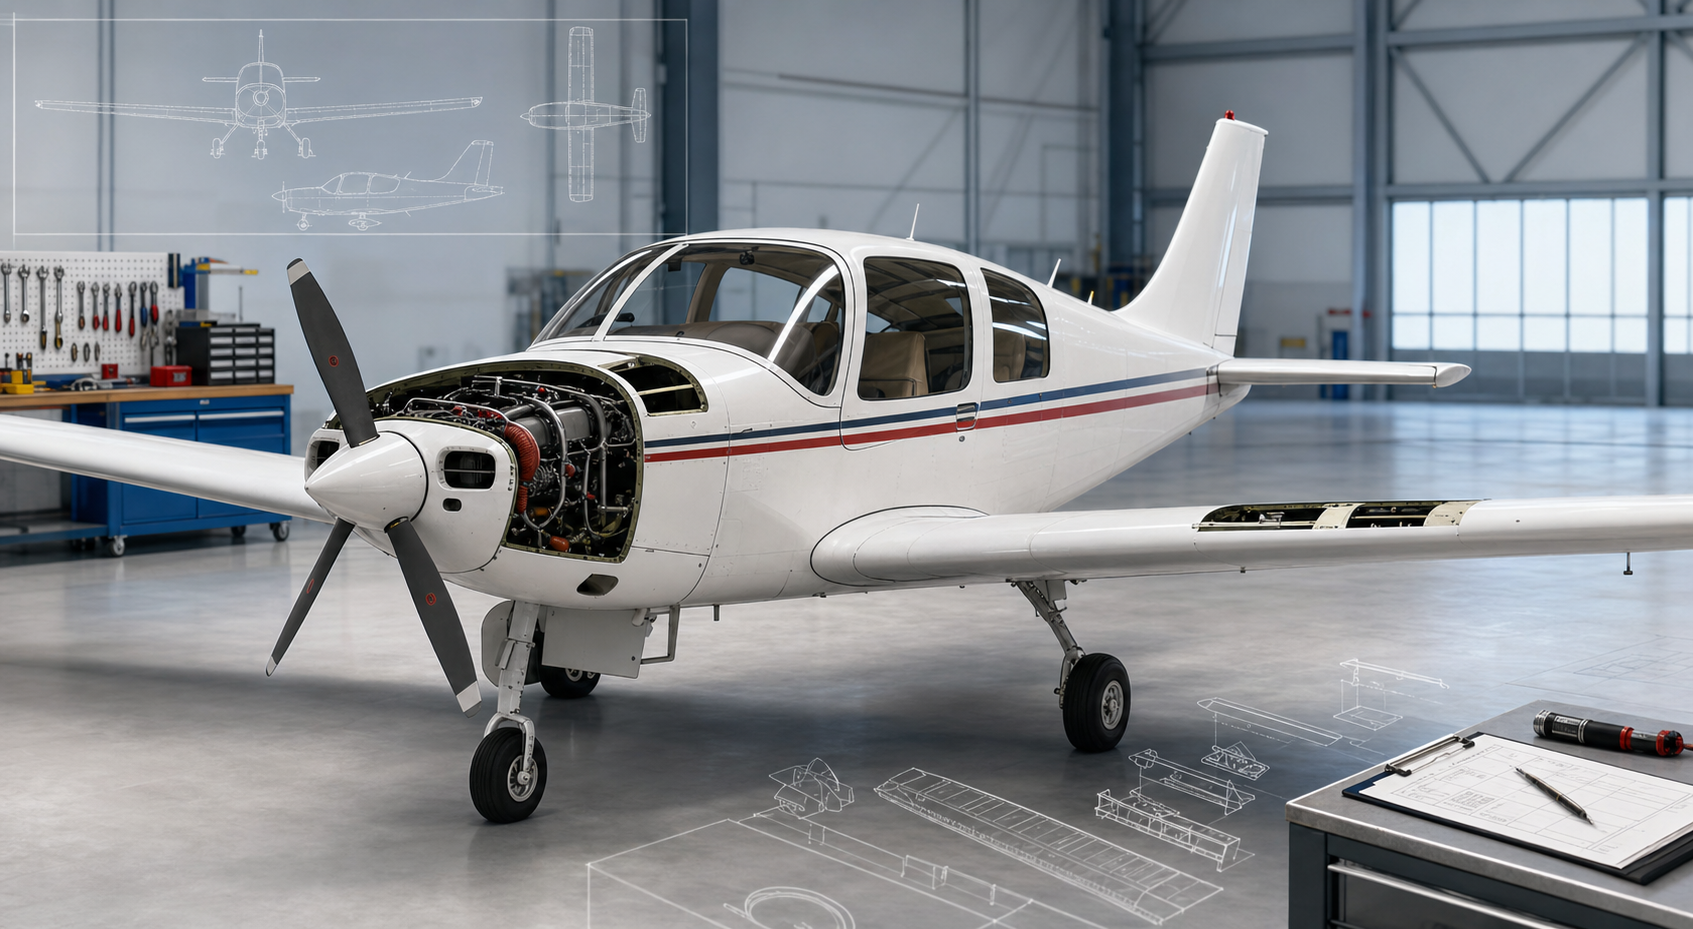
\includegraphics[width=0.95\textwidth,height=0.29\textheight,keepaspectratio]{Figuras/portada-amp.png}

        \vspace{1.0cm}

        {\fontsize{24pt}{28pt}\selectfont\bfseries \documenttitle}\\[0.25cm]
        {\fontsize{16pt}{20pt}\selectfont\bfseries \documentsubtitle}\\[0.45cm]
        {\Large \aircraft}
    \end{center}

    \vfill

    \begin{flushright}
        \large
        \begin{tabular}{@{}l@{\hspace{0.35cm}}p{0.58\textwidth}@{}}
            Efectuado por: & \groupauthors \\[5pt]
            Curso: & 2025--2026 \\[5pt]
            Fecha: & Mayo de 2026
        \end{tabular}
    \end{flushright}
\end{titlepage}

%%%%%%%%%%%%%%%%%%%%%%%%%%%%%%%%%%%%%%%%%%%%%%%%%%%%%
%%%%%%%%%%%%%%%%%%%%% Resumen %%%%%%%%%%%%%%%%%%%%%%%
%%%%%%%%%%%%%%%%%%%%%%%%%%%%%%%%%%%%%%%%%%%%%%%%%%%%%

\clearpage
\thispagestyle{empty}
\section*{Resumen}
\addcontentsline{toc}{section}{Resumen}

El presente Programa de Mantenimiento Aprobado (AMP) define las tareas de mantenimiento necesarias para asegurar la aeronavegabilidad continuada de una aeronave Socata TB 10, número de serie 649, matrícula EC-SIM, en el marco de la Parte-ML del Reglamento (UE) 1321/2014. El documento identifica la aeronave, su configuración básica, la documentación técnica empleada, los intervalos de inspección programada, las tareas especiales, los requisitos operacionales periódicos, las operaciones de servicing y los componentes sujetos a vida límite, descarte u overhaul. Asimismo, recoge las limitaciones de aeronavegabilidad y las directivas repetitivas aplicables a la célula y al motor Lycoming O-360-A1AD, dejando constancia de las limitaciones documentales existentes en el alcance académico del trabajo.

%%%%%%%%%%%%%%%%%%%%%%%%%%%%%%%%%%%%%%%%%%%%%%%%%%%%%
%%%%%%%%%%%%%%%%%%%%% Índice %%%%%%%%%%%%%%%%%%%%%%%%
%%%%%%%%%%%%%%%%%%%%%%%%%%%%%%%%%%%%%%%%%%%%%%%%%%%%%

\clearpage
\hypersetup{linkcolor=black}
\tableofcontents\thispagestyle{empty}
\hypersetup{allcolors=blue}

%%%%%%%%%%%%%%%%%%%%%%%%%%%%%%%%%%%%%%%%%%%%%%%%%%%%%%%
%%%%%%%%%%%%%%%%%%%%% Contenido %%%%%%%%%%%%%%%%%%%%%%%
%%%%%%%%%%%%%%%%%%%%%%%%%%%%%%%%%%%%%%%%%%%%%%%%%%%%%%%

\section{Introducción}
\label{sec:introduccion}

El presente Programa de Mantenimiento Aprobado (AMP) define las tareas necesarias para asegurar la aeronavegabilidad continuada de la aeronave indicada, conforme al Reglamento (UE) 1321/2014, Anexo Vb (Parte-ML), aplicable a aeronaves distintas de las complejas, operadas en categoría no comercial.

\section{Identificación de la aeronave}
\label{sec:identificacion}

\begin{table}[H]
\centering
\caption{Datos de identificación de la aeronave.}
\label{tab:identificacion-aeronave}
\renewcommand{\arraystretch}{1.25}
\begin{tabularx}{\textwidth}{|>{\bfseries\raggedright\arraybackslash}p{0.36\textwidth}|>{\raggedright\arraybackslash}X|}
\hline
Campo & Descripción \\
\hline
Fabricante & DAHER AEROSPACE / Socata \\
\hline
Modelo & TB 10 \\
\hline
Número de serie & 649 \\
\hline
Año de fabricación & 1988 \\
\hline
Matrícula & EC-SIM \\
\hline
Modelo de motor (basado en el TCDS) & Textron Lycoming O-360-A1AD \\
\hline
Modelo de hélice (basado en el TCDS) & Hartzell HC-C2YK-1BF/F 7666 A-2 \\
\hline
\end{tabularx}
\end{table}

\section{Registro de revisiones del programa}
\label{sec:registro-revisiones}

El registro de revisiones permite controlar formalmente la configuración del AMP. Cada cambio debe quedar identificado con número de revisión, fecha, motivo técnico o documental, aprobación y alcance, de forma que el propietario, CAO o CAMO pueda demostrar qué versión del programa estaba vigente y qué documentación justificó cada enmienda.

\begingroup
\small
\setlength{\tabcolsep}{4pt}
\renewcommand{\arraystretch}{1.18}
\begin{longtable}{|>{\raggedright\arraybackslash}p{0.11\textwidth}|>{\raggedright\arraybackslash}p{0.15\textwidth}|>{\raggedright\arraybackslash}p{0.52\textwidth}|>{\raggedright\arraybackslash}p{0.14\textwidth}|}
\caption{Registro de revisiones periódicas del Programa de Mantenimiento de la Aeronave.}
\label{tab:registro-revisiones}\\
\hline
\textbf{Revisión} & \textbf{Fecha} & \textbf{Motivo del cambio} & \textbf{Aprobado por} \\
\hline
\endfirsthead
\hline
\textbf{Revisión} & \textbf{Fecha} & \textbf{Motivo del cambio} & \textbf{Aprobado por} \\
\hline
\endhead
0 & 10/05/2026 & Emisión inicial del AMP académico para Socata TB 10 S/N 649. Incluye identificación de configuración, programa base, servicing, vida límite/TBO y ADs según documentación trazada. & Grupo 7 \\
\hline
1 & Reservado & Futuras enmiendas por revisión documental, cambio de configuración, AD nueva o revisada, modificación, experiencia en servicio o variación aprobada del programa. & N/A \\
\hline
\end{longtable}
\endgroup

\section{Lista de páginas efectivas (LEP)}
\label{sec:lep}

\begin{table}[H]
\centering
\caption{Lista de páginas efectivas.}
\label{tab:lep}
\renewcommand{\arraystretch}{1.2}
\begin{tabularx}{\textwidth}{|>{\raggedright\arraybackslash}X|>{\raggedright\arraybackslash}p{0.22\textwidth}|>{\raggedright\arraybackslash}p{0.18\textwidth}|}
\hline
\textbf{Sección} & \textbf{Páginas} & \textbf{Revisión} \\
\hline
Título e introducción & 1--3 & 0 \\
\hline
Identificación y revisiones & 4--5 & 0 \\
\hline
Mantenimiento programado & 6--10 & 0 \\
\hline
Desviaciones y vida límite & 11--12 & 0 \\
\hline
Declaraciones & 13 & 0 \\
\hline
\end{tabularx}
\end{table}

\begin{table}[H]
\centering
\caption{Anexos del programa.}
\label{tab:anexos}
\renewcommand{\arraystretch}{1.2}
\begin{tabularx}{\textwidth}{|>{\raggedright\arraybackslash}p{0.2\textwidth}|>{\raggedright\arraybackslash}X|>{\raggedright\arraybackslash}p{0.2\textwidth}|>{\raggedright\arraybackslash}p{0.14\textwidth}|}
\hline
\textbf{Código anexo} & \textbf{Título} & \textbf{Responsable} & \textbf{Ed/Rev} \\
\hline
Anexo 1 & Report de revisiones (Inspection Chart) & Grupo 7 & 1.0 \\
\hline
Anexo 2 & Reportes de revisión, puntos especiales y componentes con vida límite & Grupo 7 & 1.0 \\
\hline
Anexo 3 & Listado de Directivas de Aeronavegabilidad de célula & Grupo 7 & 1.0 \\
\hline
Anexo 4 & Listado de Directivas de Aeronavegabilidad de motor & Grupo 7 & 1.0 \\
\hline
Anexo 5 & Documento referencia Componentes vida límite & Grupo 7 & 1.0 \\
\hline
\end{tabularx}
\end{table}

\section*{Enmiendas, control del programa de mantenimiento y lista de distribución}
\addcontentsline{toc}{section}{Enmiendas, control del programa de mantenimiento y lista de distribución}
\label{sec:enmiendas}

Cuando sea necesario, se realizarán enmiendas a este programa de mantenimiento registrándose debidamente en la parte inicial del documento. Estas enmiendas podrán incluir cambios en las recomendaciones del titular del certificado de tipo, modificaciones, experiencia en servicio, cambios que afecten al contenido o requisitos de la autoridad competente.

Este Programa de mantenimiento se actualizará con la última edición o revisión de los manuales y documentación técnica detallada. Cuando una nueva edición o revisión de la documentación suponga una modificación de este programa se procederá a enmendar el mismo y se presentará para su aprobación en la OSV correspondiente. Para este trabajo académico, el responsable de revisión y enmienda se identifica como el grupo de trabajo; en una aeronave real correspondería al propietario, CAO/CAMO u organización responsable de aeronavegabilidad continuada.

Una vez aprobada dicha enmienda del programa, se enviará una copia actualizada a cada una de las localizaciones donde se dispone de copia del mismo.

\section{Aplicabilidad}
\label{sec:aplicabilidad}

El presente AMP aplica a aeronaves ligeras de ala fija, helicópteros o planeadores con MTOM inferior a 2730 kg, certificadas bajo EASA, operadas en categoría no comercial (Parte-ML).

\section{Utilización de la aeronave}
\label{sec:utilizacion}

Definición del rango de utilización anual normal o típico de la aeronave definido por las Instrucciones para la Aeronavegabilidad Continuada (ICA) del TCH.

La base del programa se establece considerando una utilización anual de \textbf{100 horas de vuelo/año}, \textbf{80 vuelos/ciclos/año} y \textbf{90 aterrizajes/año}, con una tolerancia del \(\pm25\%\).

En caso de desviaciones significativas, se revisará el AMP.

\noindent\textbf{Referencia ICA del TCH:} SOCATA TB 10 Maintenance Manual, Tomes 1--7, P/N Z00.18010310E0R18, Rev. 18 SEP 06, Chapter 05-20-00 (BA) ``Scheduled Inspections'', Page 1, Note 1. La nota indica que la inspección anual puede reducirse si la aeronave excede 100 \FH/año; por ello se toma 100 \FH/año como hipótesis académica de utilización normal.

\section{Base del AMP: documentos de referencia}
\label{sec:documentos-referencia}

\begingroup
\small
\setlength{\tabcolsep}{4pt}
\renewcommand{\arraystretch}{1.18}
\begin{longtable}{|>{\raggedright\arraybackslash}p{0.25\textwidth}|>{\raggedright\arraybackslash}p{0.49\textwidth}|>{\raggedright\arraybackslash}p{0.18\textwidth}|}
\caption{Documentos de referencia utilizados como base del AMP.}
\label{tab:documentos-referencia}\\
\hline
\textbf{Documento} & \textbf{Referencia} & \textbf{Edición/Fecha} \\
\hline
\endfirsthead
\hline
\textbf{Documento} & \textbf{Referencia} & \textbf{Edición/Fecha} \\
\hline
\endhead
\textbf{Manual de Mantenimiento de Aeronave (AMM)} & SOCATA TB 10 Maintenance Manual, Tomes 1--7, P/N Z00.18010310E0R18. Limitación: el TCDS EASA.A.378 exige Rev. 19 o posterior, pero no está disponible en la documentación facilitada. & Rev. 18, SEP 06 \\
\hline
\textbf{Manual de motor} & Operator's Manual Lycoming O-360, HO-360, IO-360, AIO-360, HIO-360 \& TIO-360 Series, P/N 60297-12. Aplicable a O-360-A1AD. & 8th Edition, Oct 2005; revision pages through Dec 2009 \\
\hline
\textbf{Manual de hélice} & Hartzell HC-C2YK-1BF/F 7666 A-2 referenciada por TCDS EASA.A.378, FAA TCDS P-920 y AMM. No se profundiza por indicación del profesor. & Referencia de configuración \\
\hline
\textbf{Airworthiness Limitations / Time Limits} & SOCATA TB 10 Maintenance Manual Rev. 18, Chapter 04-00-00 Airworthiness Limitations y Chapter 05-10-00 Time Limits. Limitación: el TCDS EASA.A.378 Issue 05 requiere AMM Rev. 19 o posterior con Chapter 4 Airworthiness Limitations, no disponible para este trabajo académico. & Rev. 18, SEP 06 \\
\hline
\textbf{Service Bulletins (SB) aplicables} & No se consideran otros Service Bulletins de aeronave o motor por alcance académico del trabajo. & N/A \\
\hline
\textbf{TCDS motor} & FAA TCDS E-286, Lycoming Engines O-360 series. Incluye O-360-A1AD. & Rev. 21, 30 Apr 2013 \\
\hline
\textbf{TCDS hélice} & FAA Type Certificate Data Sheet No. P-920, Hartzell HC-C2Y/BHC-C2Y/CHC-C2Y/DHC-C2Y. Incluye la combinación Hartzell HC-C2YK / F7666 con motor Lycoming O-360-A1AD. & Rev. 41, 12 Dec 2025 \\
\hline
\textbf{TBO motor} & Lycoming Service Instruction No. 1009BE, Time Between Overhaul (TBO) Schedules. O-360 except O-360-E: 2000 h. & 24 Apr 2020 \\
\hline
\end{longtable}
\endgroup

\section{Mantenimiento programado}
\label{sec:mantenimiento-programado}

\subsection{Intervalos de inspección}
\label{subsec:intervalos-inspeccion}

En este apartado se indica la relación de las inspecciones del programa base de mantenimiento, así como sus intervalos y posibles ampliaciones. Estos intervalos están establecidos de acuerdo con una utilización de la aeronave prevista en el apartado \ref{sec:utilizacion}.

\begingroup
\scriptsize
\setlength{\tabcolsep}{3pt}
\renewcommand{\arraystretch}{1.18}
\begin{longtable}{|>{\raggedright\arraybackslash}p{0.2\textwidth}|>{\raggedright\arraybackslash}p{0.22\textwidth}|>{\raggedright\arraybackslash}p{0.16\textwidth}|>{\raggedright\arraybackslash}p{0.11\textwidth}|>{\raggedright\arraybackslash}p{0.22\textwidth}|}
\caption{Inspecciones normales de mantenimiento programado.}
\label{tab:inspecciones-programadas}\\
\hline
\textbf{Inspección} & \textbf{Contenido} & \textbf{Intervalo} & \textbf{Ampliación} & \textbf{Referencia} \\
\hline
\endfirsthead
\hline
\textbf{Inspección} & \textbf{Contenido} & \textbf{Intervalo} & \textbf{Ampliación} & \textbf{Referencia} \\
\hline
\endhead
Inspección ``A'' First 25 hours & Carta de inspección inicial 25 h & 25 \FH{} iniciales & 5 \FH & SOCATA TB 10 Maintenance Manual Rev. 18, 05-20-00 (BA) Page 1--2 y 05-20-02 \\
\hline
Inspección ``2A'' / VP50 & Carta de inspección 50 h & 50 \FH{} o 6 meses, lo que antes ocurra & 5 \FH{} o 15 días & SOCATA TB 10 Maintenance Manual Rev. 18, 05-20-00 (BA) Page 1--2 y 05-20-03 \\
\hline
Inspección ``4A'' / VP100 & Carta de inspección 100 h & 100 \FH & 10 \FH & SOCATA TB 10 Maintenance Manual Rev. 18, 05-20-00 (BA) Page 1--2 y 05-20-04 \\
\hline
Inspección mayor ``80A'' & Major Inspection & 2000 \FH & N/A & SOCATA TB 10 Maintenance Manual Rev. 18, 05-20-00 (BA) Page 1 y 05-20-05 \\
\hline
Annual Inspection (AI) & Inspección anual por envejecimiento y tareas calendarizadas & 12 meses & 2 meses & SOCATA TB 10 Maintenance Manual Rev. 18, 05-20-00 (BA) Page 1 y 05-20-06 \\
\hline
\end{longtable}
\endgroup

Las tolerancias no son acumulables y el tiempo entre dos inspecciones del mismo tipo no puede exceder el intervalo más la tolerancia. Cuando existan límites por horas y calendario, aplica el que venza antes. La inspección anual se integra en el ciclo de inspecciones; si se ha realizado una inspección de 100 h en los tres meses anteriores, el AMM permite no repetir determinadas operaciones marcadas con ``0'', salvo que la inspección anual sustituya a una inspección de 100 h.

\subsection{Inspecciones especiales}
\label{subsec:inspecciones-especiales}

\begingroup
\scriptsize
\setlength{\tabcolsep}{3pt}
\renewcommand{\arraystretch}{1.18}
\begin{longtable}{|>{\raggedright\arraybackslash}p{0.22\textwidth}|>{\raggedright\arraybackslash}p{0.24\textwidth}|>{\raggedright\arraybackslash}p{0.15\textwidth}|>{\raggedright\arraybackslash}p{0.12\textwidth}|>{\raggedright\arraybackslash}p{0.18\textwidth}|}
\caption{Inspecciones especiales fuera de las revisiones estándar.}
\label{tab:inspecciones-especiales}\\
\hline
\textbf{Inspección especial} & \textbf{Contenido} & \textbf{Intervalo} & \textbf{Ampliación} & \textbf{Referencia} \\
\hline
\endfirsthead
\hline
\textbf{Inspección especial} & \textbf{Contenido} & \textbf{Intervalo} & \textbf{Ampliación} & \textbf{Referencia} \\
\hline
\endhead
Engine special inspection & Inspección especial de motor indicada por el AMM & 400 \FH & 10 \FH & SOCATA TB 10 Maintenance Manual Rev. 18, 05-20-00 (BA) Inspection Calendar; 05-20-01 Pages 234--235 \\
\hline
500 hrs special inspection & Bloque de inspección especial 500 h & 500 \FH & 50 \FH & SOCATA TB 10 Maintenance Manual Rev. 18, 05-20-00 (BA) Inspection Calendar \\
\hline
1000 hrs special inspection & Bloque de inspección especial 1000 h & 1000 \FH & 50 \FH & SOCATA TB 10 Maintenance Manual Rev. 18, 05-20-00 (BA) Inspection Calendar \\
\hline
Brake hydraulic fluid change & Cambio de fluido hidráulico de frenos & 3 años & No indicada & SOCATA TB 10 Maintenance Manual Rev. 18, 05-20-01 Page 219 \\
\hline
Fuel selector filtering element & Limpieza o sustitución del elemento filtrante del selector de combustible & 300 \FH{} o 1 año & No indicada & SOCATA TB 10 Maintenance Manual Rev. 18, 05-20-01 Page 213 \\
\hline
Flap actuator and supports & Inspección visual de fijaciones, remaches flojos y grietas & 500 \FH & No indicada & SOCATA TB 10 Maintenance Manual Rev. 18, 05-20-01 Page 212 \\
\hline
Flight control supports & Inspección visual de soportes de mandos de vuelo & 500 \FH & No indicada & SOCATA TB 10 Maintenance Manual Rev. 18, 05-20-01 Page 225 \\
\hline
Elevator hinge bearings & Inspección visual de rodamientos/bisagras de elevador & 1000 \FH{} o 2 años & No indicada & SOCATA TB 10 Maintenance Manual Rev. 18, 05-20-01 Page 227 \\
\hline
\end{longtable}
\endgroup

\subsection{Requisitos operacionales y pruebas periódicas}
\label{subsec:requisitos-operacionales}

En esta sección se registran las tareas operacionales que se controlan de forma independiente en el Excel \texttt{Tasks}, sin mezclarlas con inspecciones especiales ni con componentes de vida límite.

\begingroup
\small
\setlength{\tabcolsep}{4pt}
\renewcommand{\arraystretch}{1.18}
\begin{longtable}{|>{\raggedright\arraybackslash}p{0.24\textwidth}|>{\raggedright\arraybackslash}p{0.25\textwidth}|>{\raggedright\arraybackslash}p{0.16\textwidth}|>{\raggedright\arraybackslash}p{0.25\textwidth}|}
\caption{Requisitos operacionales y pruebas periódicas.}
\label{tab:requisitos-operacionales}\\
\hline
\textbf{Requisito / tarea} & \textbf{Descripción} & \textbf{Intervalo} & \textbf{Referencia} \\
\hline
\endfirsthead
\hline
\textbf{Requisito / tarea} & \textbf{Descripción} & \textbf{Intervalo} & \textbf{Referencia} \\
\hline
\endhead
Transponder / altimeter calibration/check & Prueba/calibración de transpondedor y altímetro & 24 meses & SOCATA TB 10 MM Rev.18, 05-10-00 p.3 / 05-20-01 p.221, 223; EASA SIB 2011-15R2 \\
\hline
Weighing and balancing & Peso y centrado & 5 años & SOCATA TB 10 MM Rev.18, 05-20-00 p.2 / 05-20-01 p.202 \\
\hline
Compass compensation & Compensación de brújula & 3 años & SOCATA TB 10 MM Rev.18, 05-20-00 p.2 / 05-20-01 p.222 \\
\hline
Air data systems tightness test & Prueba de estanqueidad del sistema de datos de aire & 300 \FH{} o 3 años & SOCATA TB 10 MM Rev.18, 05-20-01 p.222 \\
\hline
ELT visual inspection and operational test & Inspección visual y prueba operacional del ELT & 100 \FH{} o 6 meses & SOCATA TB 10 MM Rev.18, 05-20-01; control operacional independiente \\
\hline
\end{longtable}
\endgroup

\subsection{Períodos de limpieza, engrase, lubricación y relleno de fluidos}
\label{subsec:servicing}

Los periodos de inspección, limpieza, engrase, lubricación, relleno, ajuste y prueba de componentes son los incluidos en la documentación referenciada a continuación:

\begin{quote}
\raggedright
\textbf{Aircraft Maintenance Manual (AMM):} SOCATA TB 10 Maintenance Manual, P/N Z00.18010310E0R18, Rev. 18 SEP 06. Referencias principales: 05-20-01 (GA), ATA 12-10, 12-20 y ATA 20-00. Véase \texttt{trazabilidad/04\_lubricacion\_servicing.md}.
\end{quote}

\begingroup
\scriptsize
\setlength{\tabcolsep}{3pt}
\renewcommand{\arraystretch}{1.18}
\begin{longtable}{|>{\raggedright\arraybackslash}p{0.32\textwidth}|>{\raggedright\arraybackslash}p{0.21\textwidth}|>{\raggedright\arraybackslash}p{0.17\textwidth}|>{\raggedright\arraybackslash}p{0.21\textwidth}|}
\caption{Tareas de limpieza, engrase, lubricación y relleno de fluidos.}
\label{tab:servicing}\\
\hline
\textbf{Descripción} & \textbf{Intervalo} & \textbf{Ampliación} & \textbf{Referencia} \\
\hline
\endfirsthead
\hline
\textbf{Descripción} & \textbf{Intervalo} & \textbf{Ampliación} & \textbf{Referencia} \\
\hline
\endhead
Drain oil system, replace/check filter and clean crankcase strainer & First engine 10 \FH{} and 25 \FH{} or 4 months; then 50 \FH{} or 4 months & 5 \FH{} o 15 días para VP50 & SOCATA TB 10 Maintenance Manual Rev. 18, 05-20-01 (GA) Page 203, ATA 12-10 \\
\hline
Drain fuel tanks and fuel system, ventilate & Major 2000 \FH{} and Annual & 2 meses para anual & SOCATA TB 10 Maintenance Manual Rev. 18, 05-20-01 (GA) Page 203, ATA 12-10 \\
\hline
Clean exterior surface and inspect for corrosion & 100 \FH, Major 2000 \FH{} and Annual & 10 \FH{} para 100 h; 2 meses para anual & SOCATA TB 10 Maintenance Manual Rev. 18, 05-20-01 (GA) Page 203, ATA 12-20 \\
\hline
Clean engine & 100 \FH, Major 2000 \FH{} and Annual & 10 \FH{} para 100 h; 2 meses para anual & SOCATA TB 10 Maintenance Manual Rev. 18, 05-20-01 (GA) Page 203, ATA 12-20 \\
\hline
Reinforce anticorrosion protection / lubricate cockpit-fuselage and landing gear areas & 50 \FH, 100 \FH, Major 2000 \FH{} and Annual & 5 \FH/15 días para 50 h; 10 \FH{} para 100 h; 2 meses anual & SOCATA TB 10 Maintenance Manual Rev. 18, 05-20-01 (GA) Pages 203--204, ATA 20-00 \\
\hline
Reinforce anticorrosion protection / lubricate stabilizers, wings and engine compartment areas & 100 \FH, Major 2000 \FH{} and Annual & 10 \FH{} para 100 h; 2 meses anual & SOCATA TB 10 Maintenance Manual Rev. 18, 05-20-01 (GA) Page 204, ATA 20-00 \\
\hline
Lubricate bearings and wheel axles & Major 2000 \FH{} and Annual & 2 meses para anual & SOCATA TB 10 Maintenance Manual Rev. 18, 05-20-01 (GA) Page 219, ATA 32-40 \\
\hline
Lubricate door locking mechanisms & Major 2000 \FH & Regla general de tolerancias & SOCATA TB 10 Maintenance Manual Rev. 18, 05-20-01 (GA) Page 224, ATA 52-10 \\
\hline
Lubricate inside of elevator balancing boom & Major 2000 \FH & Regla general de tolerancias & SOCATA TB 10 Maintenance Manual Rev. 18, 05-20-01 (GA) Page 227, ATA 55-20 \\
\hline
\end{longtable}
\endgroup

\section{Desviaciones y justificaciones}
\label{sec:desviaciones}

Cualquier desviación del fabricante o del MIP deberá estar documentada y justificada, indicando su aprobación por CAMO/CAO o propietario responsable.

\noindent\textbf{Nota 1.} Las ampliaciones de los intervalos recomendados por \textbf{EASA} como máximos, cuando no exista indicaciones del Titular del Certificado de tipo, son los siguientes.

\noindent\textbf{Nota 2.} Como regla general, las variaciones permitidas no se aplican a \textbf{ninguna tarea obligatoria}, como por ejemplo, y de forma no exhaustiva: ADs, ALIs, LLI, CMR, FAL, Engine ALS y Aircraft Weighing.

\section{Requisitos de mantenimiento adicional}
\label{sec:mantenimiento-adicional}

Additional maintenance requirements.

\subsection{Mantenimiento debido a componentes con vida límite (life-limited components, OH/TBO)}
\label{subsec:vida-limite}

En este punto se deberán indicar aquellos componentes que tengan una vida limitada, por horas voladas, ciclos o fecha. Que bien estén sujetos a \textbf{overhaul} o a \textbf{sustitución} por \textbf{nuevo}, su intervalo especificado por el propietario del Certificado de Tipo o fabricante del componente, o la Autoridad nacional de aviación y la documentación de referencia que lo soporta.

\noindent\textbf{Nota:} No se permite ninguna variación ni extensión en los componentes para los cuales se haya prescrito una vida útil final (descarte) o un límite de revisión general (overhaul).

\begingroup
\scriptsize
\setlength{\tabcolsep}{3pt}
\renewcommand{\arraystretch}{1.18}
\begin{longtable}{|>{\raggedright\arraybackslash}p{0.25\textwidth}|>{\raggedright\arraybackslash}p{0.17\textwidth}|>{\raggedright\arraybackslash}p{0.32\textwidth}|>{\raggedright\arraybackslash}p{0.17\textwidth}|}
\caption{Componentes con vida límite, overhaul o descarte.}
\label{tab:componentes-vida-limite}\\
\hline
\textbf{Componente} & \textbf{TBO / límite} & \textbf{Documento de referencia} & \textbf{Observaciones} \\
\hline
\endfirsthead
\hline
\textbf{Componente} & \textbf{TBO / límite} & \textbf{Documento de referencia} & \textbf{Observaciones} \\
\hline
\endhead
Motor Lycoming O-360-A1AD & 2000 \FH{} o 12 años, lo que antes ocurra & Lycoming SI 1009BE, Page 2 y Table 1 Page 3; SOCATA TB 10 MM Rev. 18, 05-10-00 Page 4 & OH. No se aplica extensión TBO sin justificación específica \\
\hline
Alternator ALX 8421 / ALX 8521 / ALU 8421 & Engine overhaul & SOCATA TB 10 MM Rev. 18, 05-10-00 Page 1 & OH \\
\hline
Propeller Hartzell HC-C2YK-1BF/F7666 A-2 & Overhaul según intervalo de fabricante/regulatorio & SOCATA TB 10 MM Rev. 18, 05-10-00 Page 4 & OH. Hélice tratada a nivel suficiente por alcance académico \\
\hline
Propeller governor Hartzell F4-26 & Engine overhaul & SOCATA TB 10 MM Rev. 18, 05-10-00 Page 4 & OH \\
\hline
Carburetor Marvel 71098 MA-4-5 & Engine overhaul & SOCATA TB 10 MM Rev. 18, 05-10-00 Page 4 & OH \\
\hline
Dual magneto TCM D4LN3000 & Engine overhaul o 4 años & SOCATA TB 10 MM Rev. 18, 05-10-00 Page 4 & OH \\
\hline
Starter MZ 4222 / Lycoming LW15571 & Engine overhaul & SOCATA TB 10 MM Rev. 18, 05-10-00 Page 4 & OH \\
\hline
ELT battery assembly & 4 años o fecha límite indicada en batería & SOCATA TB 10 MM Rev. 18, 05-10-00 Pages 1--2 & Discard \\
\hline
ELT seals & 12 años & SOCATA TB 10 MM Rev. 18, 05-10-00 Page 2 & Discard \\
\hline
Fire extinguisher & 10 años; L'HOTELLIER hydrostatic test cada 5 años & SOCATA TB 10 MM Rev. 18, 05-10-00 Page 3, TR006.05 & Discard / inspection \\
\hline
Vacuum system filter AIRBORNE 1J4-7 & 500 \FH{} o 1 año & SOCATA TB 10 MM Rev. 18, 05-10-00 Page 3 & Discard \\
\hline
Emergency vacuum pump AIRBORNE 4A3-1 & 500 pump hours o 10 años & SOCATA TB 10 MM Rev. 18, 05-10-00 Page 3 & Discard \\
\hline
Access door latches TB10 25012102 & 1500 \FH & SOCATA TB 10 MM Rev. 18, 05-10-00 Page 3 & Discard \\
\hline
Teflon hoses & Unlimited & SOCATA TB 10 MM Rev. 18, 05-10-00 Pages 5--9 & On Condition \\
\hline
Fuel selector filter/drain hose TB10 52035114 & 2000 \FH{} o 10 años & SOCATA TB 10 MM Rev. 18, 05-10-00 Page 6 & Discard \\
\hline
Other elastomer/rubber/vinyl hoses & 5, 8 o 10 años según material/ubicación & SOCATA TB 10 MM Rev. 18, 05-10-00 Pages 5--9 & Discard \\
\hline
\end{longtable}
\endgroup

\subsection{Mantenimiento debido a las Instrucciones Obligatorias de Aeronavegabilidad Continua}
\label{subsec:ali-cmr}

En este punto se deberán indicar aquellas \textbf{Limitaciones Estructurales y de Aeronavegabilidad} de elementos estructurales con vida en servicio o componentes estructurales y de motor también con vida a servicio límite, con una limitación operativa por horas voladas, ciclos o calendario, que normalmente estarán sujetos a \textbf{sustitución} por \textbf{nuevo}, su intervalo especificado por el propietario del Certificado de Tipo o fabricante del componente, o la Autoridad nacional de aviación y la documentación de referencia que lo soporta.

\noindent\textbf{Nota:} No se permite ninguna variación ni extensión en los componentes para los cuales se haya prescrito una vida útil final (descarte).

La sección de limitaciones de aeronavegabilidad está aprobada por las autoridades de aeronavegabilidad: EASA especifica el mantenimiento requerido según las partes \textbf{CS23.1529} y 023.4 del Apéndice G. La sección de limitaciones de aeronavegabilidad también está aprobada por la FAA y especifica el mantenimiento requerido según las secciones \textbf{43.16 y 91.403}.

Para este trabajo académico se toma como base la documentación disponible en el cuaderno: SOCATA TB 10 Maintenance Manual Rev. 18, especialmente Chapter 04-00-00 (DC) Airworthiness Limitations y Chapter 05-10-00 Time Limits. Se deja indicada la limitación documental de que el TCDS EASA.A.378 Issue 05 requiere AMM Rev. 19 o posterior con Chapter 4 Airworthiness Limitations, no disponible en las fuentes facilitadas. Por tanto, no se aplica ninguna extensión a componentes con límite final, overhaul o descarte sin justificación específica.

\begingroup
\scriptsize
\setlength{\tabcolsep}{3pt}
\renewcommand{\arraystretch}{1.18}
\begin{longtable}{|>{\raggedright\arraybackslash}p{0.19\textwidth}|>{\raggedright\arraybackslash}p{0.26\textwidth}|>{\raggedright\arraybackslash}p{0.1\textwidth}|>{\raggedright\arraybackslash}p{0.2\textwidth}|>{\raggedright\arraybackslash}p{0.11\textwidth}|}
\caption{Limitaciones de aeronavegabilidad identificadas.}
\label{tab:ali}\\
\hline
\textbf{Elemento ALI} & \textbf{Modelo / aplicabilidad} & \textbf{Límite} & \textbf{Documento de referencia} & \textbf{Obs.} \\
\hline
\endfirsthead
\hline
\textbf{Elemento ALI} & \textbf{Modelo / aplicabilidad} & \textbf{Límite} & \textbf{Documento de referencia} & \textbf{Obs.} \\
\hline
\endhead
L.H. wing structure assembly & TB10 11000 / 11006 / 11009 series pre-MOD.152; TB10 11040 series post-MOD.152 & 14600 \FH & SOCATA TB 10 MM Rev.18, 04-00-00 (DC) Page 3 & Structure service life \\
\hline
R.H. wing structure assembly & TB10 11000 / 11006 / 11009 series pre-MOD.152; TB10 11040 series post-MOD.152 & 14600 \FH & SOCATA TB 10 MM Rev.18, 04-00-00 (DC) Page 3 & Structure service life \\
\hline
Engine mount & TB10 51000000 / 51002000; T200 51001000 / 51000000 & 10000 \FH & SOCATA TB 10 MM Rev.18, 04-00-00 (DC) Page 3 & Engine mount service life \\
\hline
Nose landing gear mount & TB10 42010001 / 42010003 / 4201000549 & 10000 \FH & SOCATA TB 10 MM Rev.18, 04-00-00 (DC) Page 3 & Landing gear mount service life \\
\hline
\end{longtable}
\endgroup

\subsection{Requisitos de mantenimiento repetitivo debido a directivas de aeronavegabilidad}
\label{subsec:ads}

Mantenimiento debido a las Directivas repetitivas de Socata \textbf{TB 10 s/n 649}: fuente FAA y EASA airworthiness directives, Service Bulletins, Modificación / STC.

\begingroup
\scriptsize
\setlength{\tabcolsep}{3pt}
\renewcommand{\arraystretch}{1.18}
\begin{longtable}{|>{\raggedright\arraybackslash}p{0.22\textwidth}|>{\raggedright\arraybackslash}p{0.16\textwidth}|>{\raggedright\arraybackslash}p{0.34\textwidth}|>{\raggedright\arraybackslash}p{0.2\textwidth}|}
\caption{Directivas repetitivas de célula.}
\label{tab:ad-celula}\\
\hline
\textbf{Referencia del documento} & \textbf{Autoridad / origen} & \textbf{Descripción} & \textbf{Periodicidad} \\
\hline
\endfirsthead
\hline
\textbf{Referencia del documento} & \textbf{Autoridad / origen} & \textbf{Descripción} & \textbf{Periodicidad} \\
\hline
\endhead
EASA AD 2007-0101 & EASA & Cabin access door hooks -- inspection/replacement, aplicabilidad condicionada a ganchos de aluminio/AU4G instalados & 110 \FH{} hasta terminating action \\
\hline
EASA AD 2015-0130 & EASA & Horizontal stabilizer spar -- special detailed inspection/corrosion protection & 72 meses \\
\hline
EASA AD 2018-0030R1 & EASA & Wing front attachments -- inspection/modification/replacement & 2000 \FH{} o 3000 \LDG, lo que antes ocurra; otras acciones según grupo/estado \\
\hline
EASA AD 2025-0160 & EASA & Lower rudder hinge fitting -- inspection & 12 meses \\
\hline
DGAC France AD F-1994-265R4 & DGAC France & Main landing gear support ribs -- inspection, aplicable si Case A & 1500 \LDG{} o 1000 \FH, lo que antes ocurra \\
\hline
DGAC France AD F-2003-368R2 & DGAC France & Flight controls gimbal joints -- aileron/elevator control inspection, si no hay terminating action & 110 \FH{} o 14 meses, lo que antes ocurra \\
\hline
\end{longtable}
\endgroup

Listado de Directivas repetitivas de \textbf{Textron Lycoming O-360-A1AD}: fuente FAA y EASA airworthiness directives, Service Bulletins, Modificación / STC.

\begingroup
\scriptsize
\setlength{\tabcolsep}{3pt}
\renewcommand{\arraystretch}{1.18}
\begin{longtable}{|>{\raggedright\arraybackslash}p{0.22\textwidth}|>{\raggedright\arraybackslash}p{0.16\textwidth}|>{\raggedright\arraybackslash}p{0.34\textwidth}|>{\raggedright\arraybackslash}p{0.2\textwidth}|}
\caption{Directivas repetitivas de motor.}
\label{tab:ad-motor}\\
\hline
\textbf{Referencia del documento} & \textbf{Autoridad / origen} & \textbf{Descripción} & \textbf{Periodicidad} \\
\hline
\endfirsthead
\hline
\textbf{Referencia del documento} & \textbf{Autoridad / origen} & \textbf{Descripción} & \textbf{Periodicidad} \\
\hline
\endhead
EASA AD 2005-0023R3 & EASA & Lycoming exhaust valve and guide inspection & 440 operating hours si no hay Hi-Chrome guides \\
\hline
FAA AD 2002-12-07 & FAA & Oil filter converter plate gasket, aplicable si motor/kit/gasket afectado & 50 h TIS hasta terminating action \\
\hline
FAA AD 2008-19-05 & FAA & ECi Titan cylinder assemblies, si cilindros afectados instalados & 50 h TIS \\
\hline
FAA AD 2009-26-12 & FAA & ECi Titan cylinder assemblies, si cilindros afectados instalados & 50 h TIS \\
\hline
FAA AD 2026-04-11 & FAA & Connecting rod bushings, si piezas afectadas instaladas & Cada oil change hasta terminating replacement \\
\hline
\end{longtable}
\endgroup

\section*{Referencias}
\addcontentsline{toc}{section}{Referencias}
\label{sec:referencias}

Basado en la Guía EASA UG.CAMO.00010-001 (2023), la Guía AESA AC-PMNA-P01-DT01 Ed.01 y la documentación técnica trazada en \texttt{trazabilidad/}.

\end{document}
